\part{APÉNDICES}
\chapter{Símbolos matemáticos} \label{simbolosmat}

\vspace{25mm}

En la siguiente página hay una imagen con los símbolos matemáticos más usados.

\vspace{45mm}
\rightline{\emph{Fuente: 3con14.com}}
\justify

\clearpage

\begin{figure}[H]
	\centering
	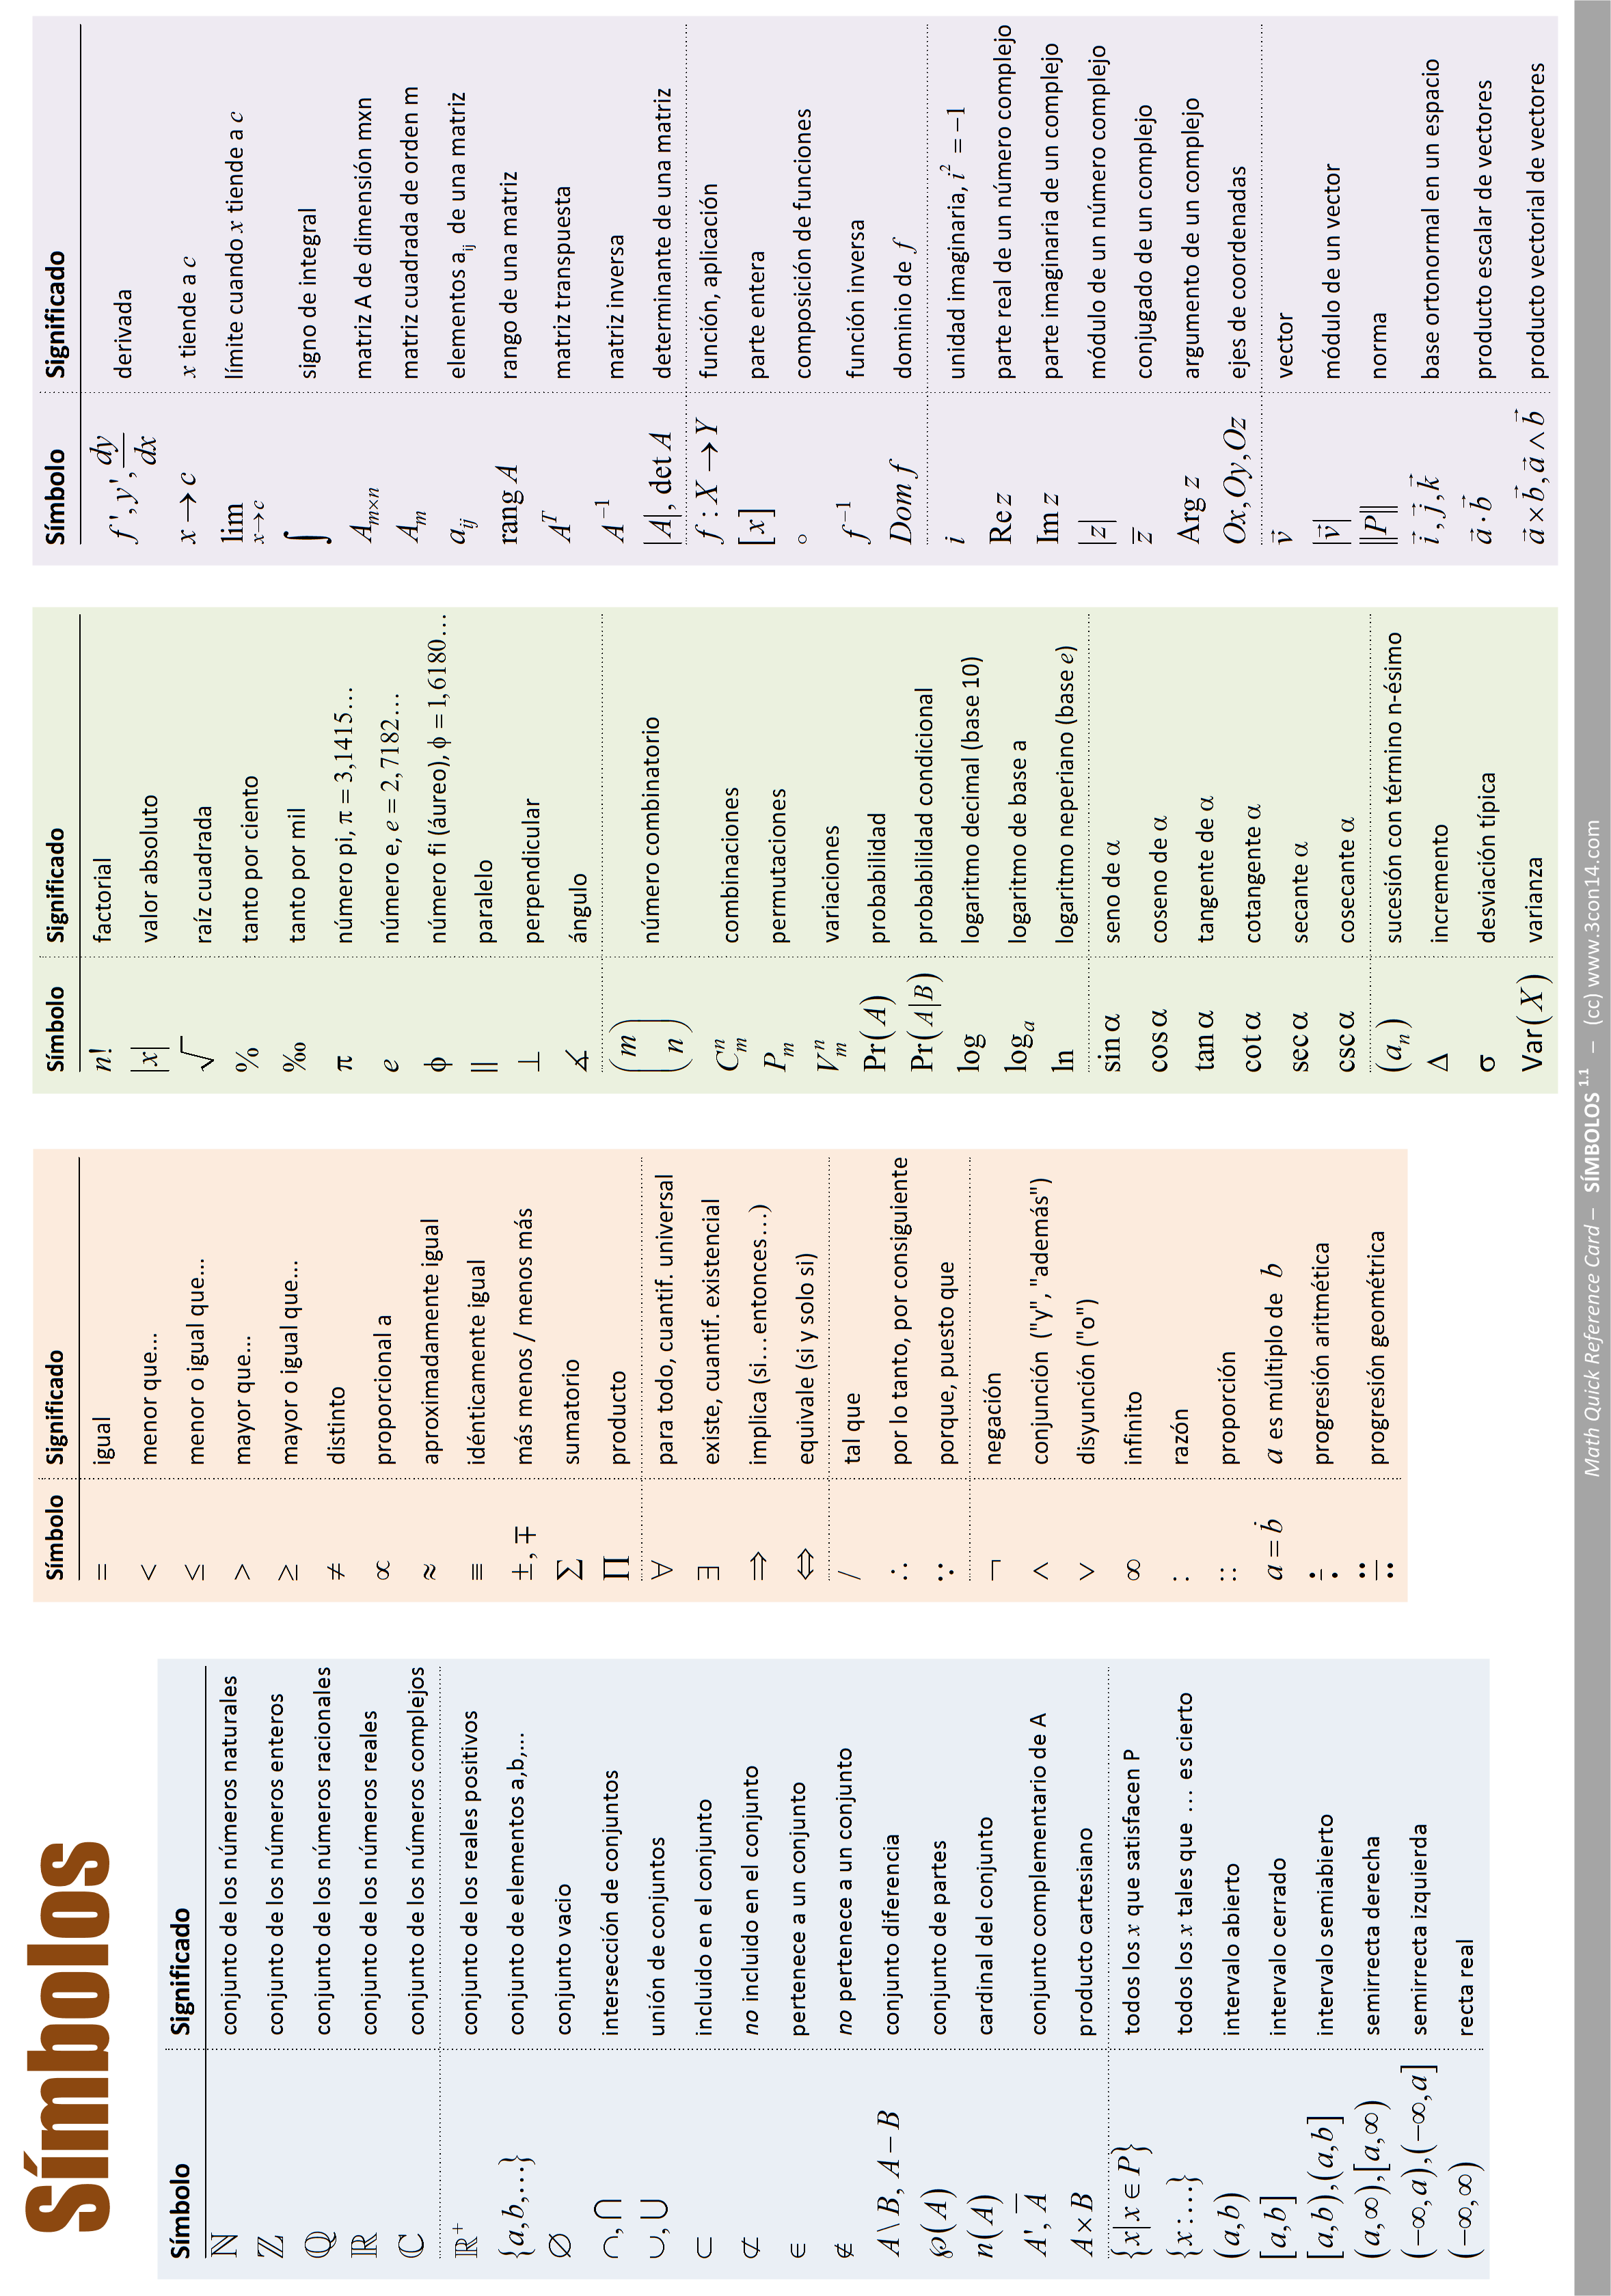
\includegraphics[width=1\textwidth]{imagenes/apendices/APENDICESIM00.png}
\end{figure}


\chapter{Sumatorios y Productorios} \label{sumatorioproductorio}

El `sumatorio' y el `productorio' son un operadores matemáticos, representados, respectivamente, por las letras griegas sigma mayúscula ($\Sigma$ correspondiente a la S latina) y pi mayúscula ($\Pi$ correspondiente a la P latina) que permiten representar de manera abreviada sumas con muchos sumandos y productos con muchos factores, con un número indeterminado (representado por alguna letra) de ellos, o incluso con infinitos. 

\section{Sumatorios}

\begin{defi}
Sea $\{a_n\}_{n\in \mathbb N}$	 una sucesión de números reales, se define:

\begin{equation*}
	\boxed{\; \sum_{i=1}^n a_i=a_1+a_2+ \cdots + a_n \; }
\end{equation*}

Si $r,s \in \mathbb N \text{ con } m\le n \to \displaystyle
\sum_{i=m}^n a_i= a_m + a_{m+1}+ a_{m+2}+ \cdots + a_m $

\end{defi}

\begin{ejem}.

	$\displaystyle \sum_{i=1}^5 i^2=1^2+2^2+3*2+4^2`5^2=1+4+9+16+25=55$
	
	$\displaystyle \sum_{i=1}^5 3=3+3+3+3+3=3\cdot 5 =15$
	
	$\displaystyle \sum_{i=3}^7 8=8+8+8+8+8=8\cdot 5=8\cdot (7-3\boldsymbol{+1})=40$
	
	$\displaystyle \sum_{i=3}^6 (2i+3)=(2(3)+3)+(2(4)+3)+(2(5)+3)+(2(6)+3)=9+11+13+15=53$
\end{ejem}

\begin{prop}{Propiedades del Sumatorio}
\begin{enumerate}
\item $\displaystyle \sum_{i=1}^n k=n\; k \qquad \qquad \sum_{i=m}^n k =(n-m+1)\; k$	
\item  $\displaystyle \sum_{i=1}^n k\; a_i= k\; \sum_{i=1}^n a_i \qquad \qquad \sum_{i=m}^n k\; a_i = k\; \sum_{i=m}^n a_i$
\item $\displaystyle \sum_{i=1}^n  (a_i\pm b_i)=\sum_{i=1}^n a_i \pm \sum_{i=1}^n b_i \qquad \qquad \cdots$
\item $\displaystyle  \sum_{i=1}^n a_i= \sum_{i=1}^m a_i + \sum_{i=m+1}^n a_i  \qquad \qquad \cdots $
\item $\displaystyle \sum_{i=1}^n (a_i-a_{i+1})=a_1-a_{n+1} \qquad \qquad 
\sum_{i=m}^n (a_i-a_{i+1})=a_m-a_{n+1}$ 

`Propiedad telescópica'.
\end{enumerate}	
\end{prop}
\begin{proof}
Las demostraciones son inmediatas teniendo en cuenta las propiedades de la suma de números reales.	
\end{proof}

\subsection{Algunos sumatorios básicos}
\begin{multicols}{2}
\begin{equation*}
	 \sum_{i=1}^n =(PA)= \dfrac {n(n+1)}{2}
\end{equation*}

\begin{equation*}
	 \sum_{i=1}^n i^2=\dfrac {n(n+1)(2n+1)}{6}
\end{equation*}

\begin{equation*}
	\sum_{i=1}^n i^3 = \left( \dfrac {n(n+1)}{2} \right) ^2
\end{equation*}

\begin{equation*}
	 \sum_{i=1}^n r^i=(PG)=\dfrac {r^{n+1}-1}{r-1}; \; r\neq 0 \wedge r\neq 1
\end{equation*}
\end{multicols}

\subsection{Doble sumatorio} Aparece con frecuencia en cálculo matricial.

$\displaystyle  \sum_{i=1}^n \left(\sum_{j=1}^n a_{ij} \right) = 
\sum_{j=1}^n a_{1j}+\sum_{j=1}^n a_{2j}+\cdots +\sum_{j=1}^n a_{nj}=$

\noindent \scriptsize{$=(a_{11}+a_{12}+\cdots +a_{1m})+(a_{21}+a_{22}+\cdots +a_{2m})+\cdots + (a_{n1}+a_{n2}+\cdots +a_{nm}) = $}

\normalsize{$\text{(reordenando)}=$}
$\displaystyle \sum_{j=1}^n \left(\sum_{i=1}^n a_{ij} \right)$

\begin{figure}[H]
	\centering
	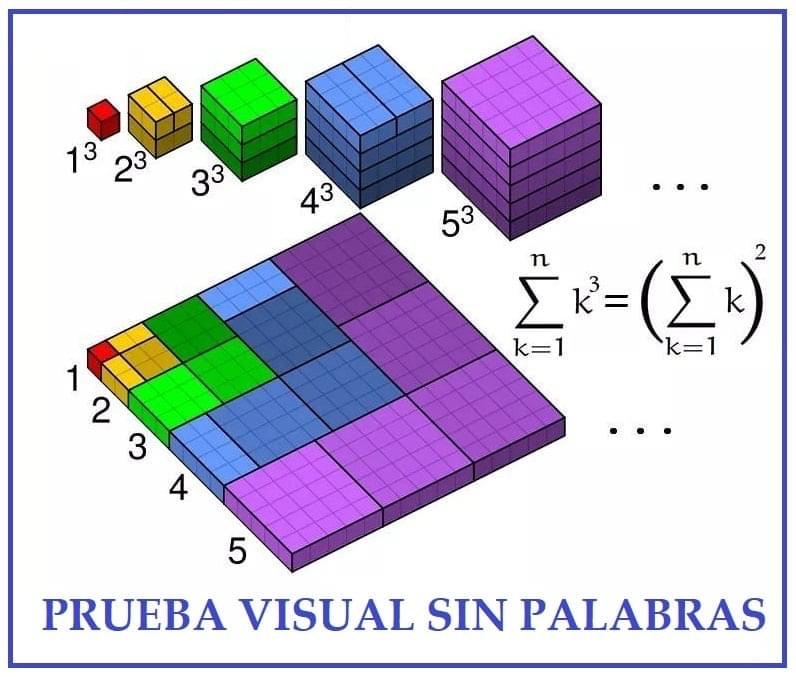
\includegraphics[width=1\textwidth]{imagenes/apendices/APENDICESIM03.png}
\end{figure}


\section{Productorios}

\begin{defi}
Sea $\{a_n\}_{n\in \mathbb N}$	 una sucesión de números reales, se define:

\begin{equation*}
	\boxed{\; \prod_{i=1}^n a_i=a_1\cdot a_2 \cdot \cdots \cdot a_n \; }
\end{equation*}

Si $r,s \in \mathbb N \text{ con } m\le n \to \displaystyle
\prod_{i=m}^n a_i= a_m \cdot  a_{m+1} \cdot  a_{m+2} \cdot \cdots \cdot a_m $

\end{defi}

\vspace{5mm} \begin{ejem}.
	
	$\displaystyle \prod_{i=1}^n i=1\cdot 2 \cdot 3 \cdot \cdots \cdot n = n!$
	
	$\displaystyle \prod_{i=3}^5 \dfrac {n+1}{n} = \dfrac {\cancel{4}}{3} \cdot \dfrac {\bcancel{5}}{\cancel{4}} \cdot \dfrac {6}{\bcancel{5}} =  \dfrac 6 3 = 2 $
	
	$\displaystyle \prod_{i=5}^8 3^{2i+1}=3^{11}\cdot 3^{13}\cdot 3^{15} \cdot 3^{17}=3^{56}$
	
\end{ejem}

\vspace{5mm} \begin{prop}{Propiedades del Productorio}

	\begin{enumerate}
	\item $\displaystyle \prod_{i=1}^n k=k^n; \quad \prod_{i=m}^n k=k^{n-m+1}$
	\item $\displaystyle \prod_{i=1}^n k \; a_i = k\; \prod_{i=1}^n a_i \qquad \qquad \cdots$
	\item $\displaystyle \prod (a_i \cdot b_i)= \prod_{i=1}^n  a_i \cdot \prod_{i=1}^n b_i \qquad \qquad \cdots$
	\item $\displaystyle \prod_{i=1}^n a_i=\prod_{i=1}^m a_i \cdot \prod_{i=m+1}^n a_i$
	
	`Propiedad telescópica'
	
	\end{enumerate}

\end{prop}

\subsection{Algunos productorios básicos}
\begin{multicols}{2}
$\displaystyle \prod_{i=1}^n k =k^n$ 

$\displaystyle \prod_{i=1}^n i =n!$

$\displaystyle \prod_{i=1}^n (i+p) = \dfrac {(n+p)!}{p!}$

$\displaystyle \prod_{i=m}^n i = \dfrac {n!}{(m-1)!}$
\end{multicols}






\chapter{El método de inducción}
\label{inducción}

		
		El \emph{Principio de inducción matemática} es un método de demostración que se usa para probar que ciertas propiedades matemáticas se verifican para todo número natural. Por ejemplo:
		
		$1^2+2^2+3^2+...+n^2=\frac 1 6 n (n+1)(2n+1)$
		
		Podemos comprobar fácilmente que se cumple esta relación para los valores $n$ concretos que se nos ocurra, pero queremos \emph{demostrar} que la relación es válida $\forall n\in \mathbb N$ y para ello usaremos el \emph{Principio de inducción matemática}, que podemos considerar como un axioma y lo entenderemos as:
		
		\begin{axio}[Principio de inducción matemática] Queremos probar que la propiedad $P(n)$ se verifica $\forall n\in \mathbb N$. Tendremos que seguir dos pasos:
			\begin{enumerate}
				\item Comprobaremos que el número 1 cumple la propiedad, es decir, $P(1)$ es cierta.
				\item Comprobaremos que si un número $n$ cumple la propiedad, \emph{entonces} también la satisface el número $n+1$. Es decir, si comprobamos que $P(n)$ es cierta, \emph{entonces} también lo es $P(n+1)$
			\end{enumerate}
			
			"Si tengo una escalera infinita y quiero poder llegar a cualquier peldaño, necesito dos cosas: un primer escalón y saber cómo dar un paso"
		\end{axio}

		
		\begin{ejem} \label{sum-cuad-induc}
		Probar que $\forall n\in \mathbb N$, se cumple:
		$1^2+2^2+3^2+...+n^2=\frac 1 6 n (n+1)(2n+1)$	
		\end{ejem}
		 Evidentemente, para $n=1$ se cumple: $1=1$
		
		\begin{proof}[Apliquemos el método de inducción.]
			
		Supongamos ahora que la propiedad es cierta para $n$, hemos de conseguir demostrar que también lo ha de ser para $n+1$, es decir, se ha de cumplir la propiedad cambiando la $n$ por $n+1$:
		
		$1^2+2^2+3^2+...+n^2+(n+1)^2=\frac 1 6 (n+1) (n+2)(2(n+1)+1)$ (*)
		
		Vamos a por ello, sumemos $(n+1)^2$ a ambos lados de la ecuación que suponemos válida para $n$:
		
		
		$1^2+2^2+3^2+...+n^2\; \; +(n+1)^2=\frac 1 6 n (n+1)(2n+1)\; \; +(n+1)^2=$
		(sacando $n+1$ factor común:)
		$=(n+1) \left( \frac 1 6 n (2n+1) +(n+1) \right)=$
		
		$=(n+1)\frac 1 6 \left(  n (2n+1) + 6(n+1) \right)=$
		$\frac 1 6 (n+1) (2n^2+7n+6)=$
		
		$=\frac 1 6 (n+1) (n+2) (2n+3)\; $ que es la expresión (*) que queramos demostrar.%$\Box$
		\end{proof}
		
		 
		Es necesario subrayar la importancia de la demostración de las dos partes del principio de inducción. Veamos un ejemplo de la importancia de la primera parte:
		
		\begin{ejem}
			Todo número natural es igual al número natural siguiente.
		\end{ejem}
		
		\begin{proof}[Mala aplicación del principio de inducción.]
			
		Aplicando la parte 2 del principio de inducción, resulta que si esto es cierto para $n$, es decir, $n=n+1$, basta con sumar $1$ a cada parte de la igualdad y escribir $n+1=n+1+1=n+2$, también será cierto para $n+1$.
		
		Obviamente la demostración no está acabada y el teorema es falso, pues falta comprobar la primera parte del método de inducción: la propiedad se cumple para $n=1$: falso, $1\neq 2$ %$\qquad \qquad \qquad \qquad \Box$
		\end{proof}
		
		Vamos a ver unos ejemplos a continuación que nos convenzan de la importancia de no quedarse con una conjetura encontrada sino que hay que demostrarla siempre.
		
		\begin{ejem}
			Sea $p(x)=x^4+x+41$, trinomio estudiado ya por Euler. Se tiene que $p(0)=41$, primo; $p(1)=43$, primo, y hasta $x=10$ se obtienen los números 47, 53, 61, 71, 83, 97, 113, 131 y 151 respectivamente, todos primos. Estaríamos tentados a afirmar que en este trinomio, al sustituir $x$ por cualquier número natural se obtiene un número primo, pero no es así, ya que, p.e., para $x=40$ tenemos $p(40)=40^2+40+41=40(40+1)+41=40\cdot 41+41=(40+1)\cdot 41=41^2$, que evidentemente no es un número primo.
		\end{ejem}
		
		 \begin{ejem} Consideremos los números de la forma $N(n)=2^{2^n}+1$. Para $n=0,1,2,3,4$ se obtienen $3, 5, 17, 257, 65537$, que son números primos. Fermat (s.XVII) aceptaba que todos los números obtenidos por esta fórmula eran primos. Fue Euler (s. XVIII) encontró $N(5)=4294967297=641\cdot 6700417$, compuesto.
		\end{ejem}
		
		\begin{ejem}
 			Leibniz (s. XVII) demostró que para cualquier número natural $n$, el número $n^3-n$ es siempre divisible por $3$, el número $n^5-n$ divisible por $5$, $n^7-n$ divisible por $7$. De ahí, supuso que si $k$ era un número natural impar, $n^k-n$ seria divisible por $k$, pero pronto observó que $2^9-2=510$ que no es divisible por $9$.
 		\end{ejem}
 		
 	    \begin{ejem}
 			$F(n)=991n^2+1$ no da nunca un cuadrado perfecto para $n=1,2,3,...$, por muchos das o años que nos dediquemos a ello. En efecto, el primer número natural para el que $F(n)$ resulta un cuadrado perfecto es:
 			
 			$n=12055735790331359447442538767.$
 		\end{ejem}
 		
 		 Con estos ejemplos podemos llegar a una sencilla pero importante conclusión: una conjetura puede ser cierta en muchos casos particulares pero si no hay demostración, nunca será un teorema.
 		 
 		 
 \chapter{Determinante de Vandermonde}
 \label{Vandermonde}
 
 \begin{multicols}{2}
Alexandre-Théophile Vandermonde (28 de febrero de 1735, París-1 de enero de 1796) fue un músico y químico francés que trabajó con Bézout y Lavoisier, aunque en la actualidad su nombre vaya principalmente asociado a la teoría de los determinantes en matemáticas. Nació y vivió toda su vida en París.

\begin{figure}[H]
	\centering
	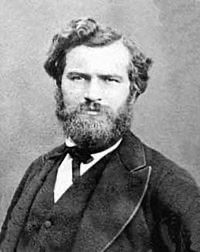
\includegraphics[width=.3\textwidth]{imagenes/apendices/APENDICESIM02.png}
\end{figure}
\end{multicols}

En este apéndice veremos una de las muchas aplicaciones de la matriz (o determinante) de Vandermonde a la interpolación polinómica.

\section{Determinante de Vandermonde de orden $n$}

\noindent Llamamos matriz de Vandermonde generada por los puntos \small{$x_0, x_1, \cdots, x_n$}\normalsize{:}

\begin{equation*}
	V(x_1,x_2,\cdots ,x_n)=
	\left( \begin{matrix}
 	1&x_0&x_0^2&\cdots &x_0^n\\
 	1&x_1&x_1^2&\cdots &x_1^n\\
 	\vdots & \vdots & \vdots & \ddots & \vdots \\
 	1&x_n&x_n^2&\cdots &x_n^n\\
 \end{matrix} \right) 
 ={[x_i^{j-1}]}_{\;i,j=1}^{\;n}
\end{equation*}

*** Determinante orden-$1$:  $det(\;V(x_1)\;)=|1|=1$

*** Determinante orden-$2$: 

$det(\; V(x_1,x_2)\; )=\left| \begin{matrix} 1&1x_1 \\ 1&x_2 \end{matrix} \right|=x_2-x_1$

*** Determinante orden-$3$:

$det(\; V(x_1,x_2,x_3)\; )=\left| \begin{matrix} 1&1x_1&x_1^2 \\ 1&x_2&x_2^2 \\1&x_3&x_3^2 \end{matrix} \right|= $ \textcolor{gris}{$\left[ \begin{matrix} C3\to C3-x_3C2 \\ C2\to C2-x_3C1 \end{matrix}  \right]=$}  

$=\left| \begin{matrix} 1&1x_1-x_3&x_1^2-x_1x_3 \\ 1&x_2-x_3&x_2^2-x_2x_3 \\1&0&0 \end{matrix} \right| = $ \textcolor{gris}{(\footnotesize{Desarrollo Laplace adjuntos última fila})} $=1\; (-1)^{3+1}\; \left| \begin{matrix} x_1-x_3&x_1^2-x_1x_3 \\ x_2-x_3&x_2^2-x_2x_3 \end{matrix} \right|=$ \textcolor{gris}{$\left[ \begin{matrix} \text{ factor común } x_1-x_3 \text { por F1 }\\\text{ factor común } x_2-x_3 \text { por F2 } \end{matrix}  \right]$} $=(x_1-x_3)(x_2-x_3) \; \left| \begin{matrix} 1&1x_1 \\ 1&x_2 \end{matrix} \right|= (x_1-x_3)(x_2-x_3)(x_2-x_1)$

*** Determinate orden-$n$:

\begin{equation*}
	det(\;V(x_1,x_2,\cdots ,x_n \;)= \prod_{1 \le i < j \le n}(x_j-x_i)
\end{equation*}

\underline{Demostración} por inducción:

--- La fórmula es correcta para $n=2$ (el caso $n=1$ es degenerado)

$det(\; V(x_1,x_2)\; )=\left| \begin{matrix} 1&1x_1 \\ 1&x_2 \end{matrix} \right|=x_2-x_1 = \prod_{i \le i < j \le 2} (x_j-x_i)$

--- Supongamos la fórmula correcta para $n-1$ y la demostraremos para $n$. Para ello usaremos la misma `astucia' que en el caso $n=3$:

\noindent (*) $C_n\to C_n-x_n C(n-1); \; \cdots ; \; C3\to C3-x_nC2; \; C2\to C2-x_n C1$:

\noindent $det(\; V(x_1,x_2, \cdots, x_n)\; )=(*)=$

\noindent $=\left| \begin{matrix}
 	1&x_1-x_x&x_1^2-x_1x_n& \cdots &x_1^{n-1}-x_1^{n-2}x_n\\
 	\vdots &\vdots & \vdots & \ddots & \vdots \\
 	1&x_{n-1}-x_n&x_{n-1}^2-x_{n-1}x_n &\cdots & x_{n-1}^{n-1}-x_{n-1}^{n-2}x_n\\ 1&0&0&\cdots &0
 \end{matrix} \right| =$

\noindent Desarrollo Laplace última fila:

\noindent $=(-1)^{n+1}
\left| \begin{matrix}
 	x_1-x_x&x_1^2-x_1x_n& \cdots &x_1^{n-1}-x_1^{n-2}x_n\\
 	\vdots & \vdots & \ddots & \vdots \\
 	x_{n-1}-x_n&x_{n-1}^2-x_{n-1}x_n &\cdots & x_{n-1}^{n-1}-x_{n-1}^{n-2}x_n
 \end{matrix} \right|$
 
 \noindent Sacamos $x_i-x_n$ de cada fila-$i$
 
 \noindent $\displaystyle =(-1)^2\cdot (-1)^{n-1}\; \prod_{1\le i < j \le n-1} (x_i-x_n)
 \left| \begin{matrix}
 1 & x_1 & x_1^2 & \cdots & x_1^{n-2}\\
 \vdots & \vdots & \ddots & \vdots \\
 1& x_{n-1} & x_{n-1}^2 & \cdots & x_{n-1}^{n-2}	
 \end{matrix} \right|=$
 
 \noindent El factor $(-1)^{n-1}$ nos permite cambiar los signos de los factores $x_i-x_n$, con $i \in \{1, \cdots, n-1\}$.
 
\noindent  Nótese que el último determinante es  $det(\; V(x_1, \cdots , x_{n-1}) \;)$. Luego:
 
 \noindent $\displaystyle det(\; V(x_1, \cdots , x_{n}) \;)= 
 \prod_{1 \le i \le n-1} (x_n-x_i) \cdot  \prod_{1 \le i < j \le n-1} (x_j-x_i)=$
 
 \noindent $=\displaystyle \prod_{1 \le j < i \le n} (x_j-x_i)$ 
 
 \rightline{$\Box$}




\section{Polinomio interpolador}

En la interpolación lineal se parte de $n$-puntos iniciales: 

\centerline{$(x_0,y_0),\; (x_1,y_1),\; \cdots ,\; (x_n,y_n)$, }

y nuestro objetivo consiste en encontrar un polinomio de grado $\le n$: 

\centerline{$\ P(x)=a_0+a_1x+a_2x^2+ \cdots + a_nx^n$}

que pase poe esos puntos, es decir, que cumpla  $n+1$ condiciones:

\centerline{$P(x_k)=y_k,\; \forall k \in \{0,1,2,\cdots,n\}$}

Si los valors de $x_k$ son distintos, entonces se puede garantizar que existe un único polinomio de grado $\le n$ que cumple las condiciones fijadas (pasar por los $n+1$ puntos).

Si los valores $x_0, x_1, \cdots , x_n$ están ordenados 
($x_0 < x_1 < \cdots < x_n$), podemos usar el polinomio encontrado, `polinomio
interpolador' para calcular el valor de $y$ en posiciones intermedias de $x$ dentro del intervalo de interpolación, $[x_0,x_n]$.


\section{Matriz de Vandermonde}

Para encontrar el polinomio interpolador hay que resolver un sistema de $n+1$ ecuaciones lineales con $n+1$ incógnitas (SEL):

--- $n+1$ puntos: $(x_0,y_0),\; (x_1,y_1),\; \cdots ,\; (x_n,y_n)$

--- Polinomio a determinar: $\ P(x)=a_0+a_1x+a_2x^2+ \cdots + a_nx^n$

--- $n+1$ condiciones: $P(x_k)=y_k,\; \forall k \in \{0,1,2,\cdots,n\}$

Entonces, se tiene el siguiente SEL:

\begin{equation*}
	\left( \begin{matrix}
 	1&x_0&x_0^2&\cdots &x_0^n\\
 	1&x_1&x_1^2&\cdots &x_1^n\\
 	\vdots & \vdots & \vdots & \ddots & \vdots \\
 	1&x_n&x_n^2&\cdots &x_n^n\\
 \end{matrix} \right) \cdot
 \left( \begin{matrix}
 	a_0\\a_1\\ \vdots \\a_n
 \end{matrix} \right) =
 \left( \begin{matrix}
 	y_0\\y_1\\ \vdots \\y_m
 \end{matrix} \right)
\end{equation*}


La matriz de los coeficientes se llama `matriz de Vandermonde' asociada a los puntos $x_0, x_1, x_2, \cdots, x_n$. Es una matriz cuadrada de orden $n+1)$.

Si en la solución del sistema se usa la regla de Cramer, el denominador de las incógnitas sería el determinante de Vandermonde que vimos, para orden cuatro en uno de los ejercicios resueltos del tema de determinantes.

\begin{equation*}
	\boxed{\; \; 
	V(x_0, x_1, x_2, \cdots, x_n)=
	\left( \begin{matrix}
 	1&x_0&x_0^2&\cdots &x_0^n\\
 	1&x_1&x_1^2&\cdots &x_1^n\\
 	\vdots & \vdots & \vdots & \ddots & \vdots \\
 	1&x_n&x_n^2&\cdots &x_n^n\\
 \end{matrix} \right) \; \; }
\end{equation*}

\section{Ejemplo}

\begin{multicols}{2}
Consideremos la siguiente tabla de valores:

\begin{table}[H]
\centering
\begin{tabular}{|c|c|c|c|c|}
\hline
x & -1 & 1/2 & 1 & 2 \\ \hline
y & 1  & 2   & 0 & 3 \\ \hline
\end{tabular}
\end{table}
\end{multicols}

La matriz de Vandermonde correspondiente a las abcisas $x_0=-1; \; x_1=1/2; \; x_2=1; \; x_3=2$ es:

\begin{equation*}
	V=
	\left( \begin{matrix}
 	1&-1&1&-1\\
 	1&1/2&1/4&1/8 \\
 	1&1&1&1 \\
 	1&2&4&8
 \end{matrix} \right) 
\end{equation*}

El polinomio interpolador de grado $\le 3$ será de la forma:

\vspace{2mm} \centerline{$P(x)=a_0+a_1x+a_2x^2+a_3x^3$}

Los coeficientes $a_k$ se obtienen al resolver el sistema:

\begin{equation*}
	\left( \begin{matrix}
 	1&-1&1&-1\\
 	1&1/2&1/4&1/8 \\
 	1&1&1&1 \\
 	1&2&4&8
 \end{matrix} \right) \cdot
 \left( \begin{matrix}
 	a_0\\a_1\\ a_2 \\a_3
 \end{matrix} \right) =
 \left( \begin{matrix}
 	1\\2\\ 0 \\3
 \end{matrix} \right)
\end{equation*}

La solución del mismo es: $a_0=4; \; a_1=-17/6; \; a_2=-7/2; \; a_3=7/3$, con lo que el polinomio interpolador es:

\begin{equation*}
P(x)=4-\dfrac {17}{6} x -\dfrac 7 2 x^2+\dfrac 7 3 x^3	
\end{equation*},

que permite aproximar el valor de $y=P(x)$ para cualquier $x\in[-1,2]$



\vspace{10mm}


\noindent \scriptsize{\emph{Fuente: Francisco Palacios. Escuela Politécnica Superior de Ingeniería Manresa. Universidad Politécnica de Catalunya. Dep. Matemática Aplicada III. Abril 2008}}\normalsize{.}



\chapter{Vectores en diferentes sistemas de coordenadas}
\chaptermark{Vectores $\neq$ Sist. Coord.}
 \label{VectoresDistintosSistemasCoordenadas}

En coordenadas cartesianas o rectangulares, las componentes del vector de posición de un punto $P(x,y,z)$ son: $\boldsymbol{ \vec r}=\overrightarrow{\mathcal O P}=\boldsymbol{ x\vec i+y\vec j+ z \vec k}$

\section{Sistema de coordenadas cilíndricas}

La posición de un punto $P$ viene dado, en cilíndricas, por dos distancias y un ángulo $P(r,\theta,z)$ y los vectores unitarios son $\overrightarrow{u_r}$,  $\overrightarrow{u_{\theta}}$, $\vec k$.


El vector unitario $\vec k$ , se aplica en el punto $P$ y es paralelo al eje $OZ$.

El vector unitario $\overrightarrow{u_r}$ se aplica en $P$ y es paralelo al vector $\vec r$ dibujado en el plano $XY$, estando determinado por la proyección de $P$ sobre el citado plano.

El vector unitario $\overrightarrow{u_{\theta}}$ se aplica en $P$ y es perpendicular a los otros dos verificando $\vec k \times \overrightarrow{u_r}=\overrightarrow{u_{\theta}}$.

El vector de posición de un punto $P$ viene determinado por $\vec R=r \vec u_r+z\vec k$, no quedando unívocamente determinado.


\begin{figure}[H]
	\centering
	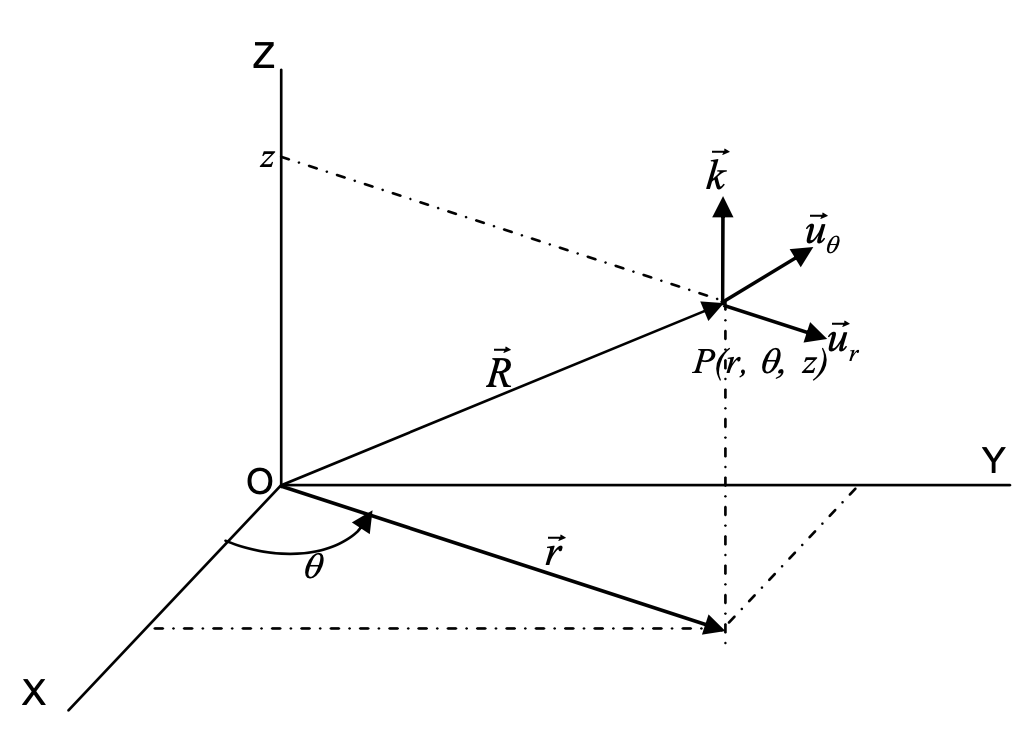
\includegraphics[width=.9\textwidth]{imagenes/apendices/APENDICESIM04.png}
\end{figure}


RELACIÓN DE LOS SISTEMAS DE COORDENADAS CILÍNDRICAS Y RECTANGULARES.

Buscamos las relaciones de $\overrightarrow{u_r}$, $\overrightarrow{u_{\theta}}$ con los vectores $\vec i$ y $\vec j$, pues $\vec k$ es el mismo en ambos sistemas de coordenadas. Para ello, trasladamos $\overrightarrow{u_r}$ y $\overrightarrow{u_{\theta}}$ al plano $XY$:

\begin{figure}[H]
	\centering
	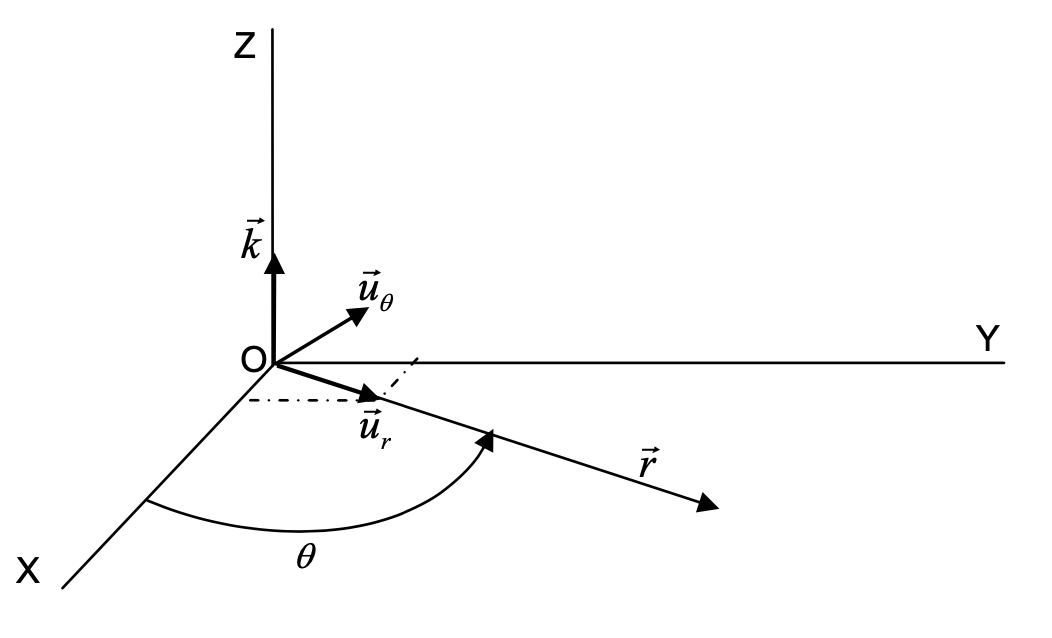
\includegraphics[width=.9\textwidth]{imagenes/apendices/APENDICESIM04b.png}
\end{figure}

Como $\overrightarrow{u_r}$ y $\overrightarrow{u_{\theta}}$  son unitarios $\to \abs{\overrightarrow{u_r}}=\abs{\overrightarrow{u_{\theta}}}=1$ 

$$ \overrightarrow{u_r}= \cos \theta \vec i + \sin \theta \vec j$$
$$ \overrightarrow{u_{\theta}}=\cos \left(\theta+\dfrac \pi 2 \right) \vec i + \sin \left(\theta+\dfrac \pi 2 \right) \vec j=-\sin \theta \vec i + \cos \theta \vec j$$
$$\vec k=\vec k$$

\begin{ejem}
	Un punto tiene por coordenadas cartesianas $P(4,3,2)$, ¿cuáles son sus coordenadas cilíndricas?
\end{ejem}
$\abs{\vec r}=\sqrt{4^2+3^2}=5 \quad \to \quad P_C=r\vec \;{u_r} + z \; \vec k = 5\; \vec {u_r}+2 \; \vec k$
\vspace{5mm}\begin{ejem}
Expresa el vector $\vec v=-8\vec i+10\vec j-12\vec k$ en coordenadas cilíndricas si su punto de aplicación está en $P(4,3,2$	
\end{ejem}
Calculemos primero los vectores unitarios $\overrightarrow{u_r}$, $\overrightarrow{u_{\theta}}$, $\vec k$ en el punto $P(4,3,2)$:


$\cos \theta=x/r=4/5=0.8; \quad \sin \theta=y/r=3/5=0.6$

$\overrightarrow{u_r} =\cos \theta \vec i + \sin \theta \vec j=0.8\vec i + 0.6 \vec j$, 

$\overrightarrow{u_{\theta}}=\-sin \theta \vec i + \cos \theta \vec j=-0.6\vec i + 0.8 \vec j$

\vspace{2mm}Para expresar $\vec v$ en cilíndricas, $\vec {v_C}$, hemos de calcular sus componentes en las direcciones de $\overrightarrow{u_r}$, $\overrightarrow{u_{\theta}}$y $\vec k$  que no es más que la proyección del vector sobre los vectores unitarios, que por serlo, coincide con el producto escalar ($\vec i$, $\vec j$, $\vec k$ forman una BON):

\vspace{2mm} $\vec v \cdot \vec {u_r}=(-8\vec i +10\vec j-12 \vec k)\cdot (0.8\vec i + 0.6 \vec j)=-6.4+6=-0.4$

$\vec v \cdot \vec {u_{\theta}}=(-8\vec i +10\vec j-12 \vec k)\cdot (-0.6\vec i + 0.8 \vec j)=4.8+8=12.8$

$\vec v \cdot \vec k=(-8\vec i +10\vec j-12 \vec k)\cdot (1\vec k)=-12$


Por lo que: $\quad \vec {a_C}=-0.4\; \vec {u_r}+12.8\; \vec {u_{\theta}}-12\; \vec k$

Compruébese que $\abs{\vec {v_c}}=\sqrt{308}=\abs{\vec v}$. El módulo es el mismo, obviamente, independientemente del sistema de coordenadas elegido.

\section{Sistema de coordenadas esféricas}
La posición de un punto $P$ queda determinado por una distancia $r$ y dos ángulos $\theta$ y $\phi$, $P(r,\theta,\phi)$.  Los vectores unitarios son $\vec u_{r}$ $\vec u_{\theta}$, $\vec u_{\phi}$.

\begin{figure}[H]
	\centering
	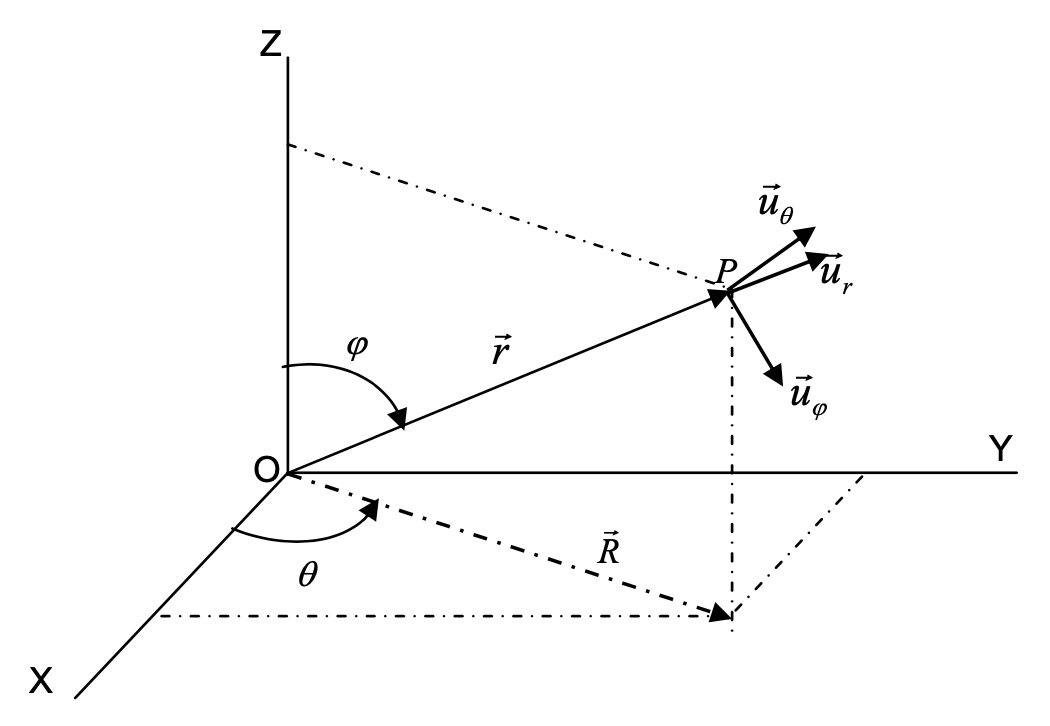
\includegraphics[width=.9\textwidth]{imagenes/apendices/APENDICESIM05.png}
\end{figure}

El vector director $\vec u_{r}$ está en la dirección $\overrightarrow{OP}=\vec r$.

l vector unitario $\vec u_{\phi}$ es perpendicular a $\vec u_{r}$ y su sentido es aquel en que $\phi$ crece.

l vector unitario $\vec u_{\theta}$ es perpendicular a los dos anteriores verificándose: $\vec u_{r} \times \vec u_{\phi} = \vec u_{\theta}$.

Un punto $P$ tiene un vector de posición que se encuentra en la dirección $OP$. En esféricas: $\vec r=r\; \vec u_r$ . No determina unívocamente su posición, solo indica que $P$ está a distancia $r$ del origen.


RELACIÓN DE LOS SISTEMAS DE COORDENADAS ESFÉRICAS Y RECTANGULARES.

\begin{figure}[H]
	\centering
	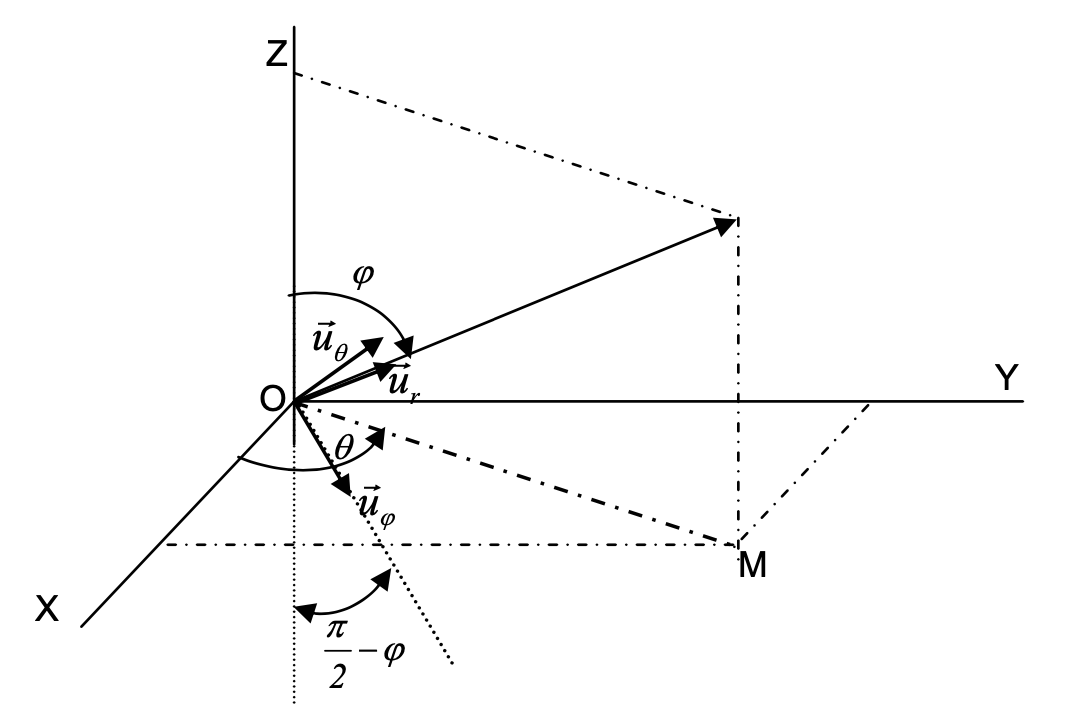
\includegraphics[width=.9\textwidth]{imagenes/apendices/APENDICESIM05b.png}
\end{figure}
Buscaremos las relaciones entre los vectores unitarios $\vec u_{r}$, $\vec u_{\theta}$, $\vec u_{phi}$ y los $\vec i$, $\vec j$, $\vec k$. Trasladamos los vectores unitarios al origen para facilitar el cálculo.

El vector $\vec u_{r}$ debe proyectarse previamente sobre el plano $XY$, dirección $OM$, antes de hacerlo sobre los ejes $X$ e $Y$. Esta proyección vale $\abs{\vec u_r} \sin \phi=1\; \sin \phi=\sin \phi$. Para proyectar $\vec {u_{\phi}}$  observamos que forma con el eje $Z$ un ángulo $(\frac \pi 2 - \phi)$ pero también debe ser proyectado antes sobre el plano $XY$ y después sobre los ejes.

Para proyectar $\vec {u_{\theta}}$ vemos que forma con el eje $X$, un ángulo $(\theta + \frac \pi 2)$.


$$\vec {u_r}=\sin \phi \cos \theta \;\vec i + \sin \phi \sin \theta \;\vec j + \cos \phi \; \vec k$$

$$\vec {u_{\phi}}=\sin (\frac \pi 2 -\phi) \cos \theta \; \vec i +\sin (\frac \pi 2 -\phi) \sin \theta \; \vec j - \cos (\frac \pi 2 - \phi)\; \vec k =$$ 
$$= \cos \phi \cos \theta \; \vec i + \cos \phi \sin \theta \; \vec j - \sin \phi \; \vec k$$

$$\vec {u_{\theta}}= \cos (\frac \pi 2 + \theta)\; \vec i + \sin (\frac \pi 2 + \theta)\; \vec j+0; \vec k = -\sin \theta \; \vec i + \cos \theta \vec j $$

\begin{ejem}
	Un punto tiene por coordenadas cartesianas $P(4,3,2)$, expresar su vector de posición en coordenadas esféricas.
\end{ejem}

$\abs{\vec r)}=\sqrt{4^2+3^2+2^2}=\sqrt{29};\qquad \vec r = r\; \vec u_r=29\; \vec u_r$

\begin{ejem}
	Expresar el vector $\vec v=-8\vec i+10 \vec j - 12 \vec k$ en coordenadas esféricas si su punto de aplicación está en $P(4,3,2)$.
\end{ejem}

Calculemos los vectores unitarios $\vec u_{r}$ $\vec u_{\theta}$, $\vec u_{\phi}$ en el punto $P(4,3,2)$. Obsérvese el vector $\vec R$ de la figura anterior a la anterior.

$\abs{\vec R}=\sqrt{4^2+3^2}=5; \quad \cos \theta =4/5=0.8;\quad \sin \theta=3/5=0.6;\quad \cos \phi=2/\sqrt{29};\quad \sin \phi=5/\sqrt{29}$

$$\vec u_r=\dfrac 5 {\sqrt{29}}\cdot 0.8 \; \vec i+\dfrac 5 {\sqrt{29}}\cdot 0.6 \; \vec j + \dfrac 2 {\sqrt{29}}\; \vec k = \dfrac  1{\sqrt{29}}\; (4\vec i+3\vec j+2\vec k)$$

$$ \vec {u_{\phi}}=\dfrac 2 {\sqrt{29}}\cdot 0.8 \;  \vec i + \dfrac 2 {\sqrt{29}}\cdot 0.6 \; \vec j - \dfrac 5 {\sqrt{29}}\; \vec k =
	\dfrac  1{\sqrt{29}}\; (1.6\vec i+1.2\vec j-5\vec k)$$

$$\vec {u_{\theta}}=-0.6\vec i+0.8 \vec j$$

Calcularemos las componentes del vector a$\vec v$ en las direcciones de los vectores unitarios $\vec u_{r}$ $\vec u_{\theta}$, $\vec u_{\phi}$ multiplicando escalarmente el vector por cada uno de estos unitarios.

$$ \vec v \cdot \vec {u_{r}}= (-8,10,-12)\cdot \frac 1 {\sqrt{29}} (4,3,2)=\frac {-26}{\sqrt{29}}$$ 

$$ \vec v \cdot \vec {u_{\phi}}= (-8,10,-12)\cdot \frac 1 {\sqrt{29}} (1.6,1.2,-5)=\frac {59.2}{\sqrt{29}}$$

$$ \vec v \cdot \vec {u_{\theta}}= (-8,10,-12)\cdot \frac 1 {\sqrt{29}} (-0.6,0.8,0)=12.8$$

Por lo que $\quad \vec {v_E}=\frac {-26}{\sqrt{29}}\; \vec {u_{r}}+ \frac {59.2}{\sqrt{29}}\; \vec {u_{\phi}}+ 12.8\; \vec {u_{\theta}}$.

\newpage %*************************************
\chapter*{} 
 
$\quad$ 
	